%% The "\appendix" call has already been made in the declaration
%% of the "appendices" environment (see thesis.tex).
\chapter{Pointless extras}
\label{app:Pointless}

\chapter{Single Parameter Variations}\label{app:single_parameter_variations}

\def\proposalxsec{
genie_ccresAxial_Genie,genie_ncresAxial_Genie,genie_qema_Genie,genie_NC_Genie,genie_NonResRvpCC1pi_Genie,genie_NonResRvnCC1pi_Genie,genie_NonResRvbarnCC1pi_Genie,genie_NonResRvbarpCC1pi_Genie,genie_NonResRvpCC2pi_Genie,genie_NonResRvnCC2pi_Genie,genie_NonResRvbarnCC2pi_Genie,genie_NonResRvbarpCC2pi_Genie,genie_NonResRvpNC1pi_Genie,genie_NonResRvnNC1pi_Genie,genie_NonResRvbarnNC1pi_Genie,genie_NonResRvbarpNC1pi_Genie,genie_NonResRvpNC2pi_Genie,genie_NonResRvnNC2pi_Genie,genie_NonResRvbarnNC2pi_Genie,genie_NonResRvbarpNC2pi_Genie}

\def\modernxsec {genie_DISAth_Genie,genie_DISBth_Genie,genie_DISCv1u_Genie,genie_DISCv2u_Genie,genie_IntraNukeNabs_Genie,genie_IntraNukeNcex_Genie,genie_IntraNukeNinel_Genie,genie_IntraNukeNmfp_Genie,genie_IntraNukeNpi_Genie,genie_IntraNukePIabs_Genie,genie_IntraNukePIcex_Genie,genie_IntraNukePIinel_Genie,genie_IntraNukePImfp_Genie,genie_IntraNukePIpi_Genie,genie_ResDecayGamma_Genie,genie_ccresVector_Genie,genie_cohMA_Genie,genie_cohR0_Genie,genie_ncelAxial_Genie,genie_ncelEta_Genie,genie_ncresVector_Genie}


\def\uncorrflux  {horncurrent_FluxUnisim,expskin_FluxUnisim,nucleoninexsec_FluxUnisim,nucleontotxsec_FluxUnisim,nucleonqexsec_FluxUnisim,pioninexsec_FluxUnisim, piontotxsec_FluxUnisim,pionqexsec_FluxUnisim}


\begin{figure}
\centering
\foreach \x in \uncorrflux{
\begin{subfigure}[p]{0.185\textwidth}
    \includegraphics[width =\textwidth]{figures-chap6/tweak_nsigma_nue/\x_nuelikeCChigh_3sigma_\x.png}
\end{subfigure}
}
\caption[Flux systematic parameter validation.]{A comparison of the +3$\sigma$ variations from the response functions used by VALOR and the universes for the complete set of uncorrelated flux systematic parameters.}
\end{figure}

\begin{figure}
\centering
\foreach \x in \proposalxsec{
\begin{subfigure}[p]{0.185\textwidth}
    \includegraphics[width =\textwidth]{figures-chap6/tweak_nsigma_nue/\x_nuelikeCChigh_3sigma_\x.png}
\end{subfigure}
}
\caption[Proposal interaction systematic parameter validation.]{A comparison of the +3$\sigma$ variations from the response functions used by VALOR and the universes for the complete set of proposal interaction systematic parameters.}
\end{figure}


\begin{figure}
\centering
\foreach \x in \modernxsec{
\begin{subfigure}[p]{0.185\textwidth}
    \includegraphics[width =\textwidth]{figures-chap6/tweak_nsigma_nue/\x_nuelikeCChigh_3sigma_\x.png}
\end{subfigure}
}
\caption[Modern interaction systematic parameter validation.]{A comparison of the +3$\sigma$ variations from the response functions used by VALOR and the universes for the complete set of modern cross-section systematic parameters.}
\end{figure}

\chapter{Detector Volumes}
\label{app:Detector_Volumes}


\begin{table}[h!]
%\begin{tabular}{lR{15}cc}
\begin{tabular}{lccc}
 & \multicolumn{1}{c}{X [cm]} & \multicolumn{1}{c}{Y [cm]} & \multicolumn{1}{c}{Z [cm]} \\ \cline{2-4} 
 & \multicolumn{3}{c}{Active Volume} \\ \cline{2-4} 
SBND & -199.15 -- \phantom{-}199.15 & -200.00 -- 200.00 & \phantom{-00}0.00 -- \phantom{0}500.00 \\
MicroBooNE & \phantom{00}-1.55 -- \phantom{-}254.80 & -115.53 -- 117.47 & \phantom{-00}0.10 -- 1036.90 \\
ICARUS Module 1 & -364.49 -- \phantom{0}-67.94 & -173.41 -- 143.41 & -909.95 -- \phantom{0}879.95 \\
ICARUS Module 2 & \phantom{-0}67.94 -- \phantom{-}364.49 & -173.41 -- 143.41 & -909.95 -- \phantom{0}879.95 \\ \cline{2-4} 
 & \multicolumn{3}{c}{Fiducial Volume} \\ \cline{2-4} 
SBND TPC 1 & -190.90 -- \phantom{-00}5.60 & -185.00 -- 185.00 & \phantom{-0}15.00 -- 415.00 \\
SBND TPC 2 & \phantom{-0}10.90 -- \phantom{-}190.90 & -185.00 -- 185.00 & \phantom{-0}15.00 -- 415.00 \\
MicroBooNE & \phantom{00}-1.55 -- \phantom{-}229.80 & \phantom{0}-90.53 -- \phantom{0}92.47 & \phantom{-0}30.10 -- 986.90 \\
ICARUS TPC 1 & -339.49 -- -221.04 & -148.41 -- 118.41 & -879.95 -- 829.95 \\
ICARUS TPC 2 & -218.89 -- \phantom{0}-92.94 & -148.41 -- 118.41 & -879.95 -- 829.95 \\
ICARUS TPC 3 & \phantom{-0}92.94 -- \phantom{-}211.39 & -148.41 -- 118.41 & -879.95 -- 829.95 \\
ICARUS TPC 4 & \phantom{-}214.39 -- \phantom{-}339.39 & -148.41 -- 118.41 & -879.95 -- 829.95
\end{tabular}
\caption[The active and fiducial volumes of the \gls{sbn} detectors.]{The dimensions defining the active and fiducial volumes for each \gls{sbn} detector using their respective coordinate systems.} \label{table:active_and_fiducial_volumes}
\end{table}

\chapter{Reconstruction Performance}
\label{app:reconstruction_performance}

The figures in \ChapterRef{chap:Energy_Reco} showing the reconstruction performance were produced whilst running Pandora in cheating mode in order to decouple the reconstruction methods from inefficiencies within the pattern recognition. If Pandora is instead used without cheating mode enabled, the resolution of the reconstruction algorithms is expected to worsen owing to the fact that the number of hits associated with true and reconstructed information is no longer in perfect agreement. 

With cheating mode no longer enabled in Pandora, the true vs reconstructed energy is shown for all three planes using the ESTAR method in \FigureRef{fig:ESTAR_true_vs_reco_no_cheat}. The fractional resolution from the collection plane is shown in \FigureRef{fig:frac_res_no_cheat} for all three reconstruction methods.

\begin{figure}[h!]
    \centering
    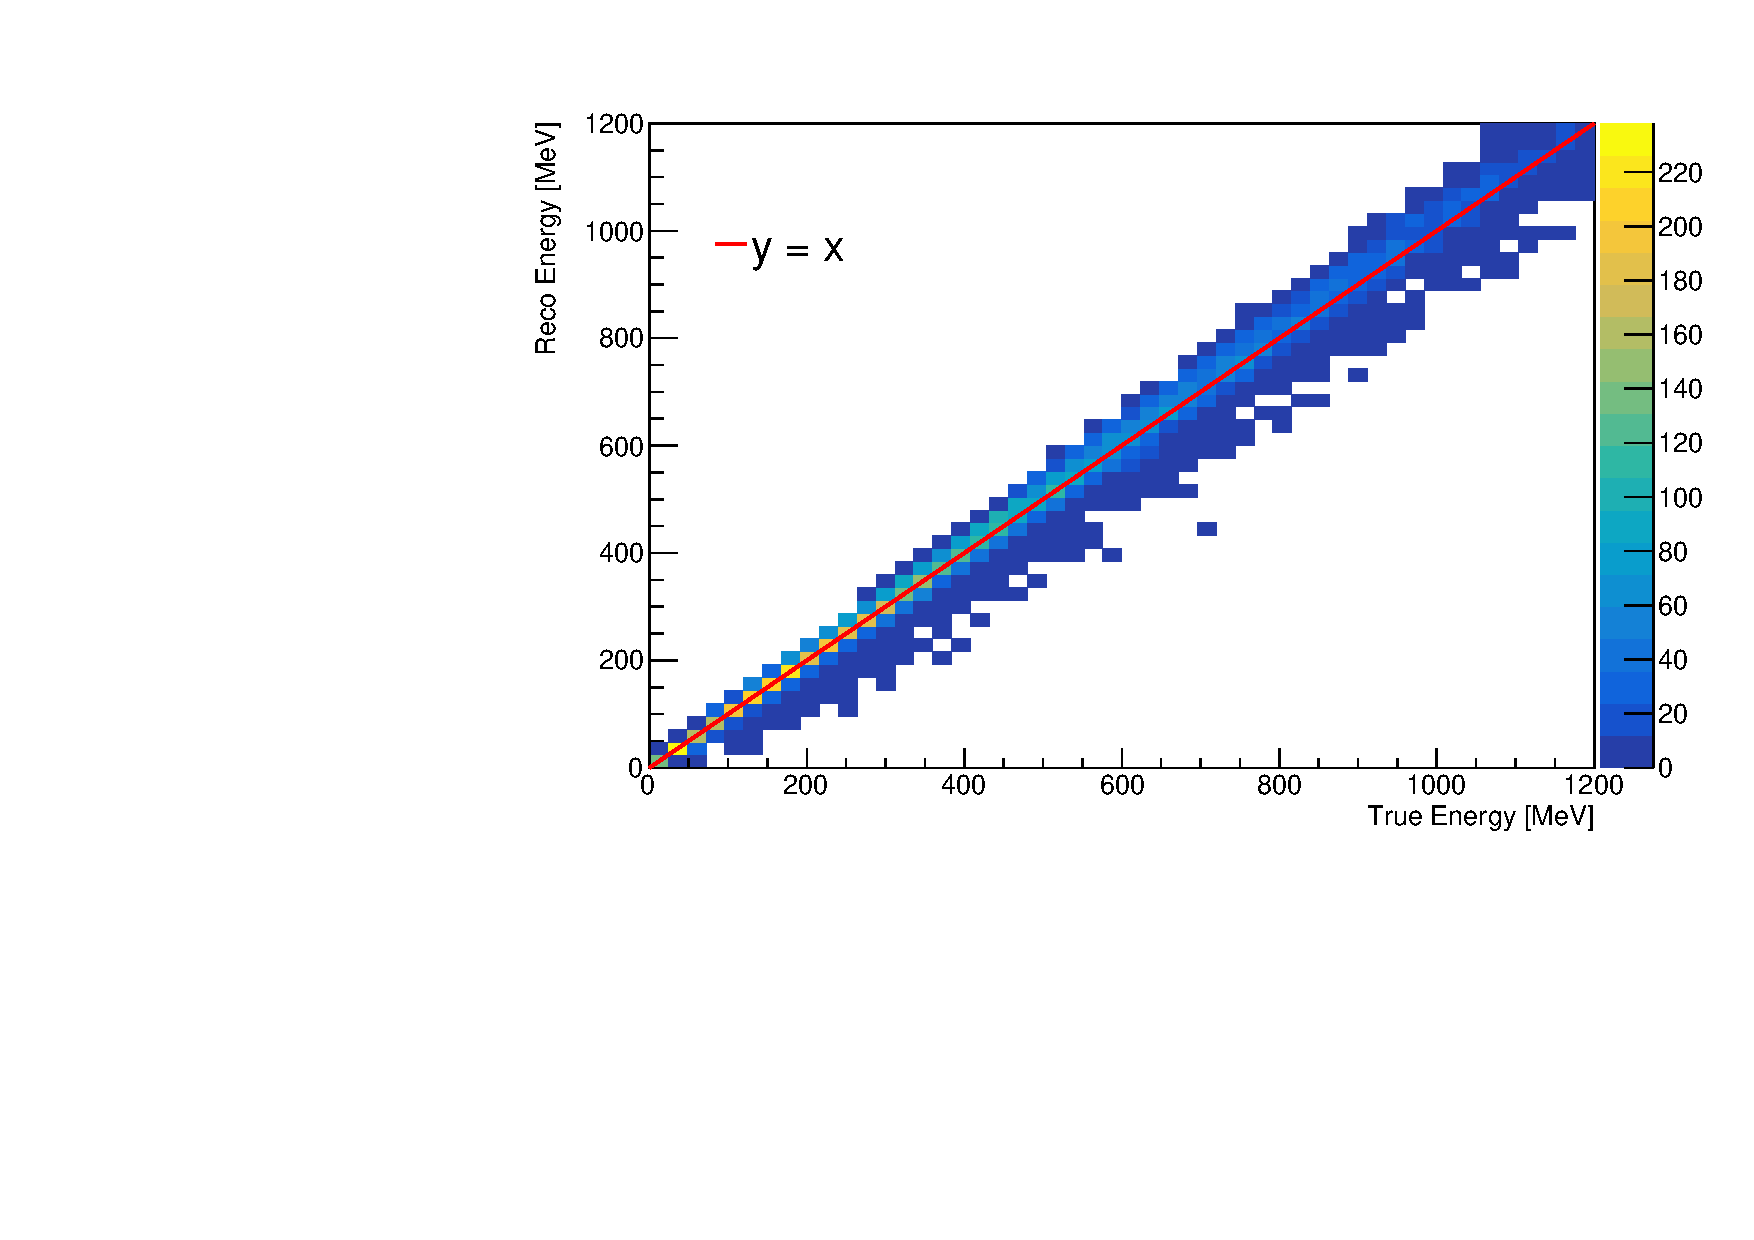
\includegraphics[width = 0.49\textwidth]{figures-chap4/non_cheat/ESTAR_plane0_true_vs_reco.pdf}
    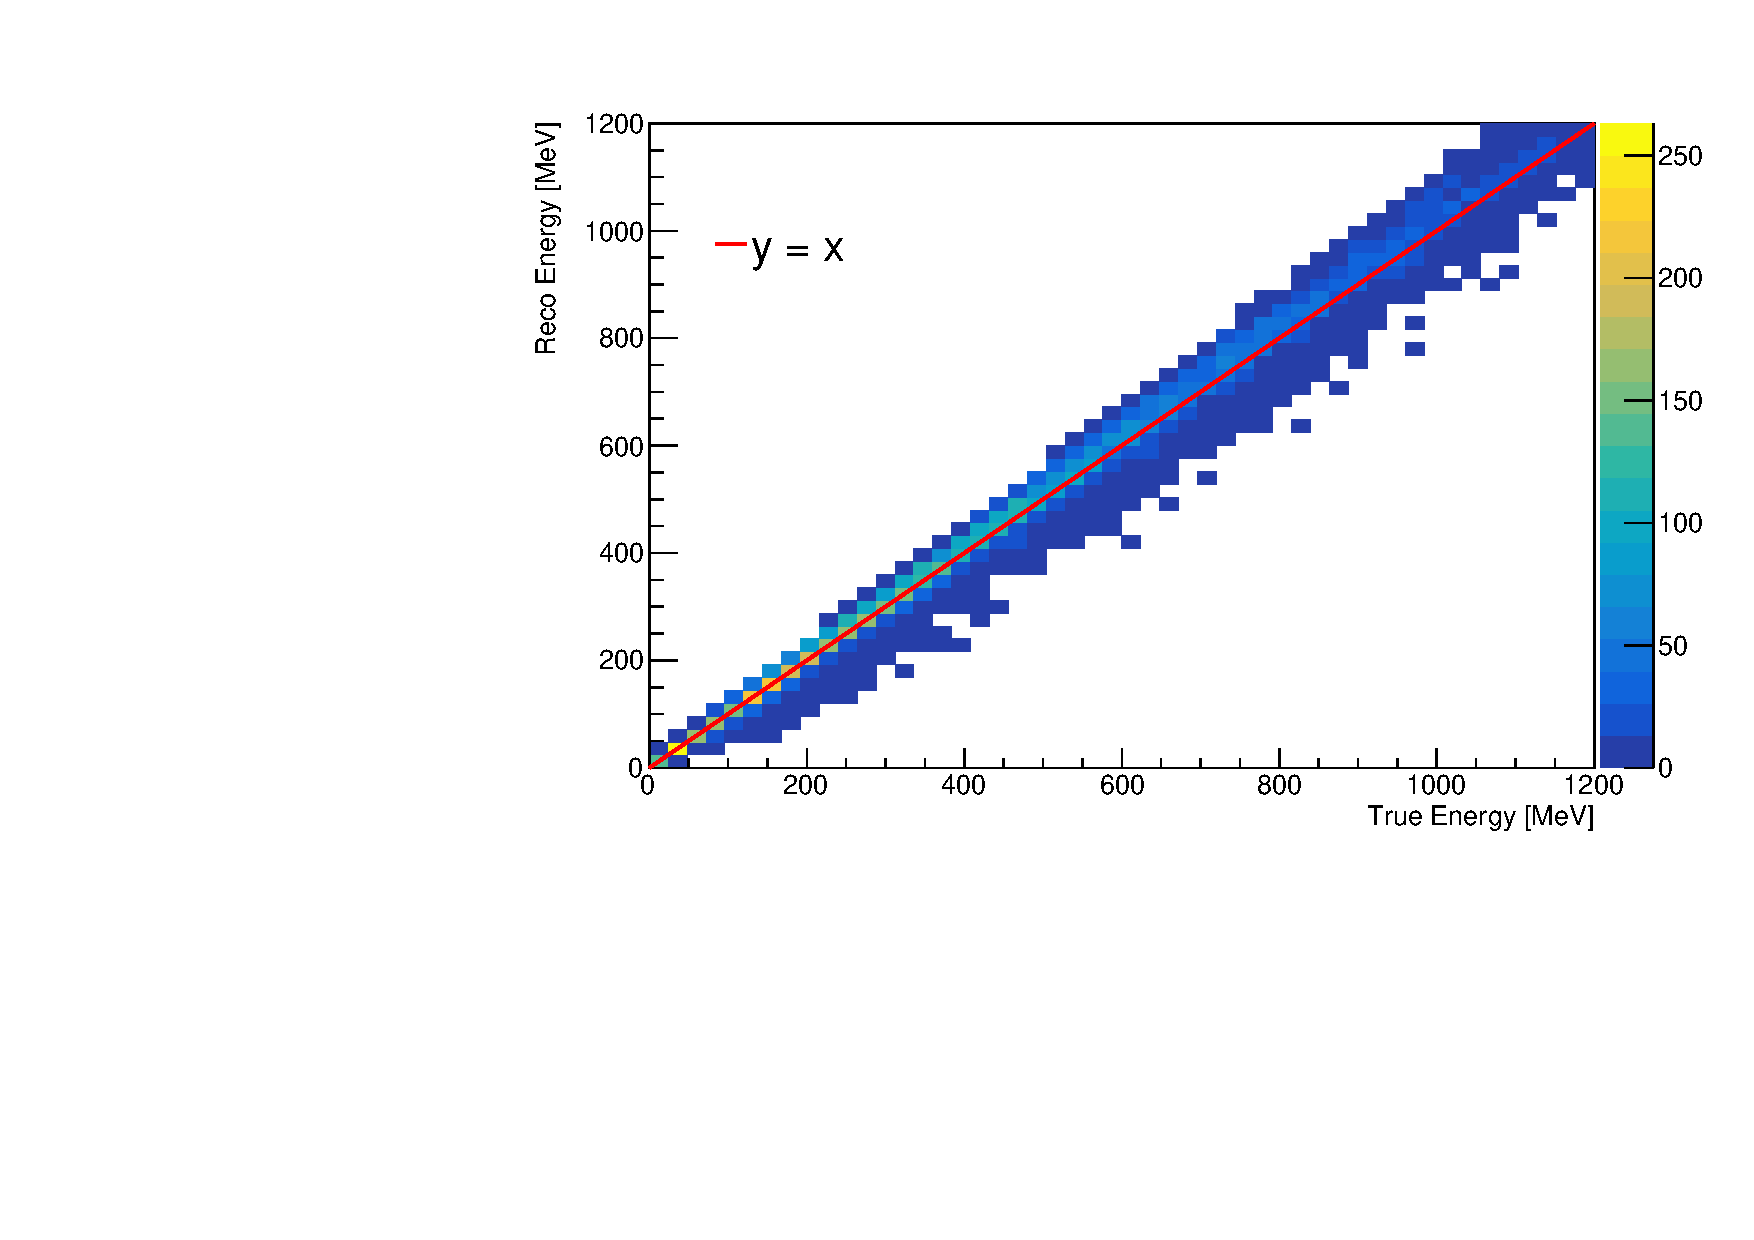
\includegraphics[width = 0.49\textwidth]{figures-chap4/non_cheat/ESTAR_plane1_true_vs_reco.pdf}
    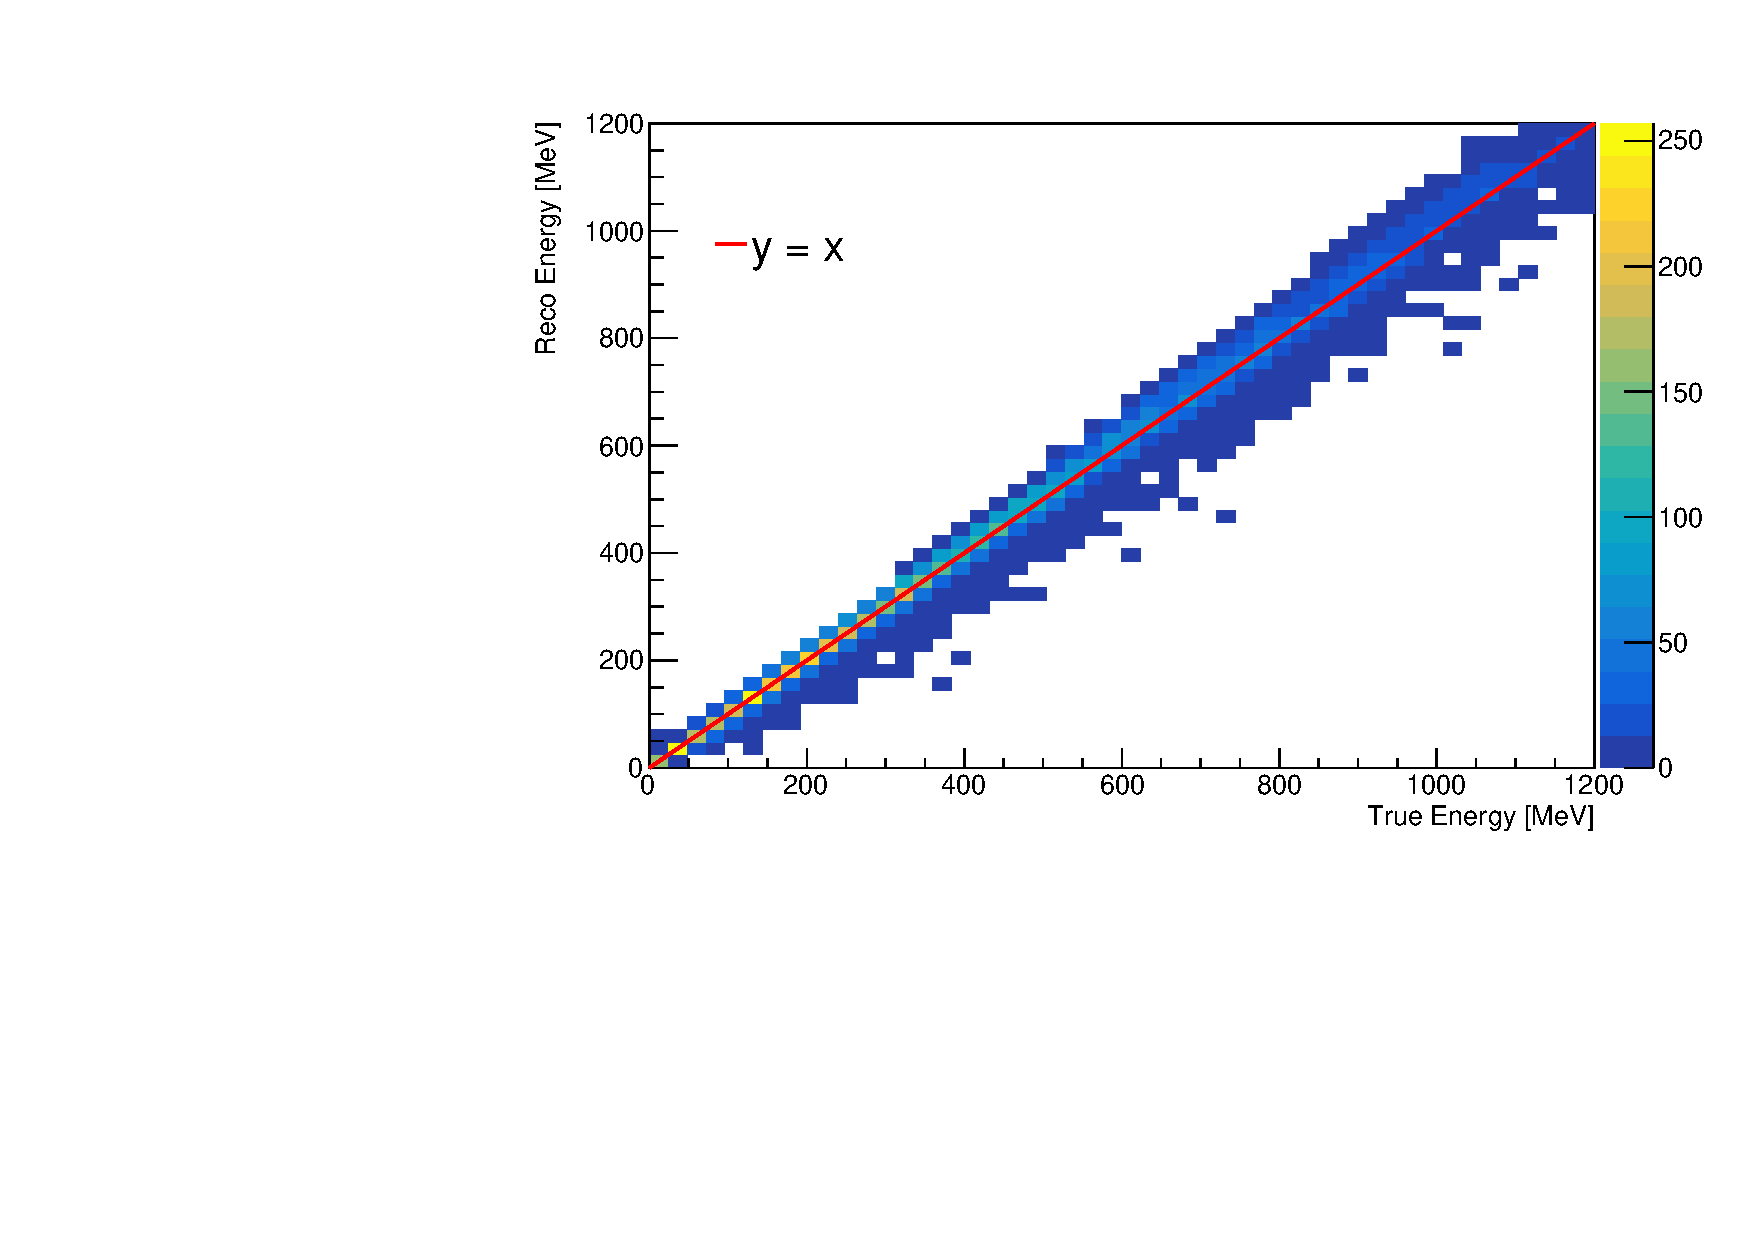
\includegraphics[width = 0.49\textwidth]{figures-chap4/non_cheat/ESTAR_plane2_true_vs_reco.pdf}
    \captionsetup{width=0.45\textwidth}
    \parbox[b]{0.49\textwidth}%
    {
    \caption[True vs reconstructed energy from the ESTAR method without using Pandora in cheating mode.]
    {True vs reconstructed energy from a showering electron. The true energy has been evaluated from the hits of each shower. Pandora was not run in cheating mode. Top Left: Induction plane 0, Top Right: Induction plane 1 and Bottom Left: Collection plane. \\}
    \label{fig:ESTAR_true_vs_reco_no_cheat}}
\end{figure}

\begin{figure}[h!]
    \centering
    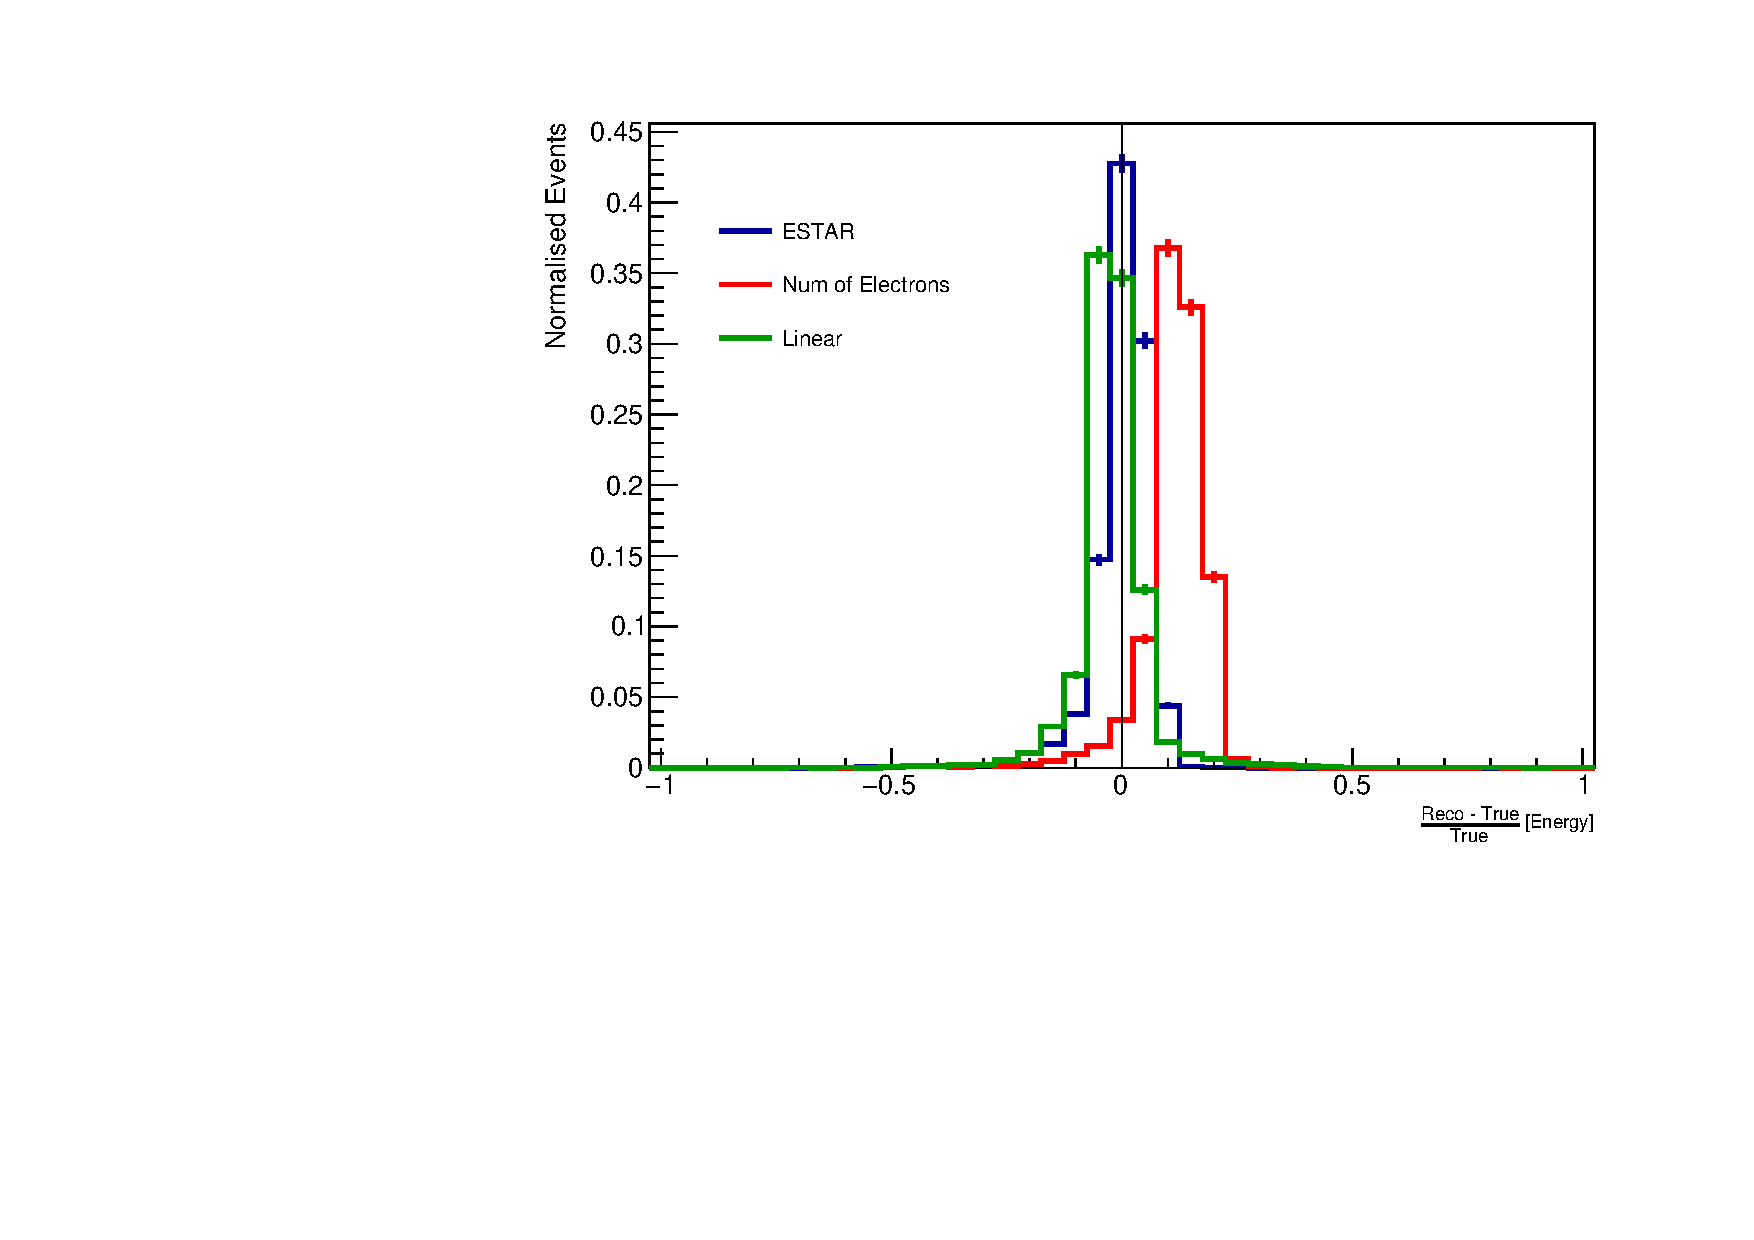
\includegraphics[width = \largefigwidth]{figures-chap4/non_cheat/ESTAR_plane2_frac_res.pdf}
    \caption[Fractional resolution of the shower energy with Pandora being run not in cheating mode.]{Comparison of the fractional energy resolution from a showering electron for the Shower Linear Energy tool, the Shower Num Electrons Energy tool and the Shower ESTAR Energy tool. The true energy is taken to be the true energy of the available hits and for the reconstruction, Pandora was run whilst not in cheating mode.}
    \label{fig:frac_res_no_cheat}
\end{figure}

Comparing \FigureRef{fig:ESTAR_true_vs_reco_no_cheat} to the ESTAR plot in \FigureRef{fig:reco_vs_true_hit_level} and \FigureRef{fig:true_vs_reco_for_induction_planes}, it can be seen that the resolution has degraded by disabling cheating mode in Pandora. Similarly, in \FigureRef{fig:frac_res_no_cheat}, each of the distributions has a noticeable tail in the negative x-direction which isn't present in the distributions shown in \FigureRef{fig:fractional_energy_resolution}.

%% Big appendixes should be split off into separate files, just like chapters
%\input{app-myreallybigappendix}
